\begin{appendices}
    \chapter{Öldaten}
    % ----------------------------------------
    % Chap: Oil daten
    % ----------------------------------------
        % ----------------------------------------
        % Fig: FVA chemische Öldaten
        % ----------------------------------------
        \begin{figure}
            \centering
            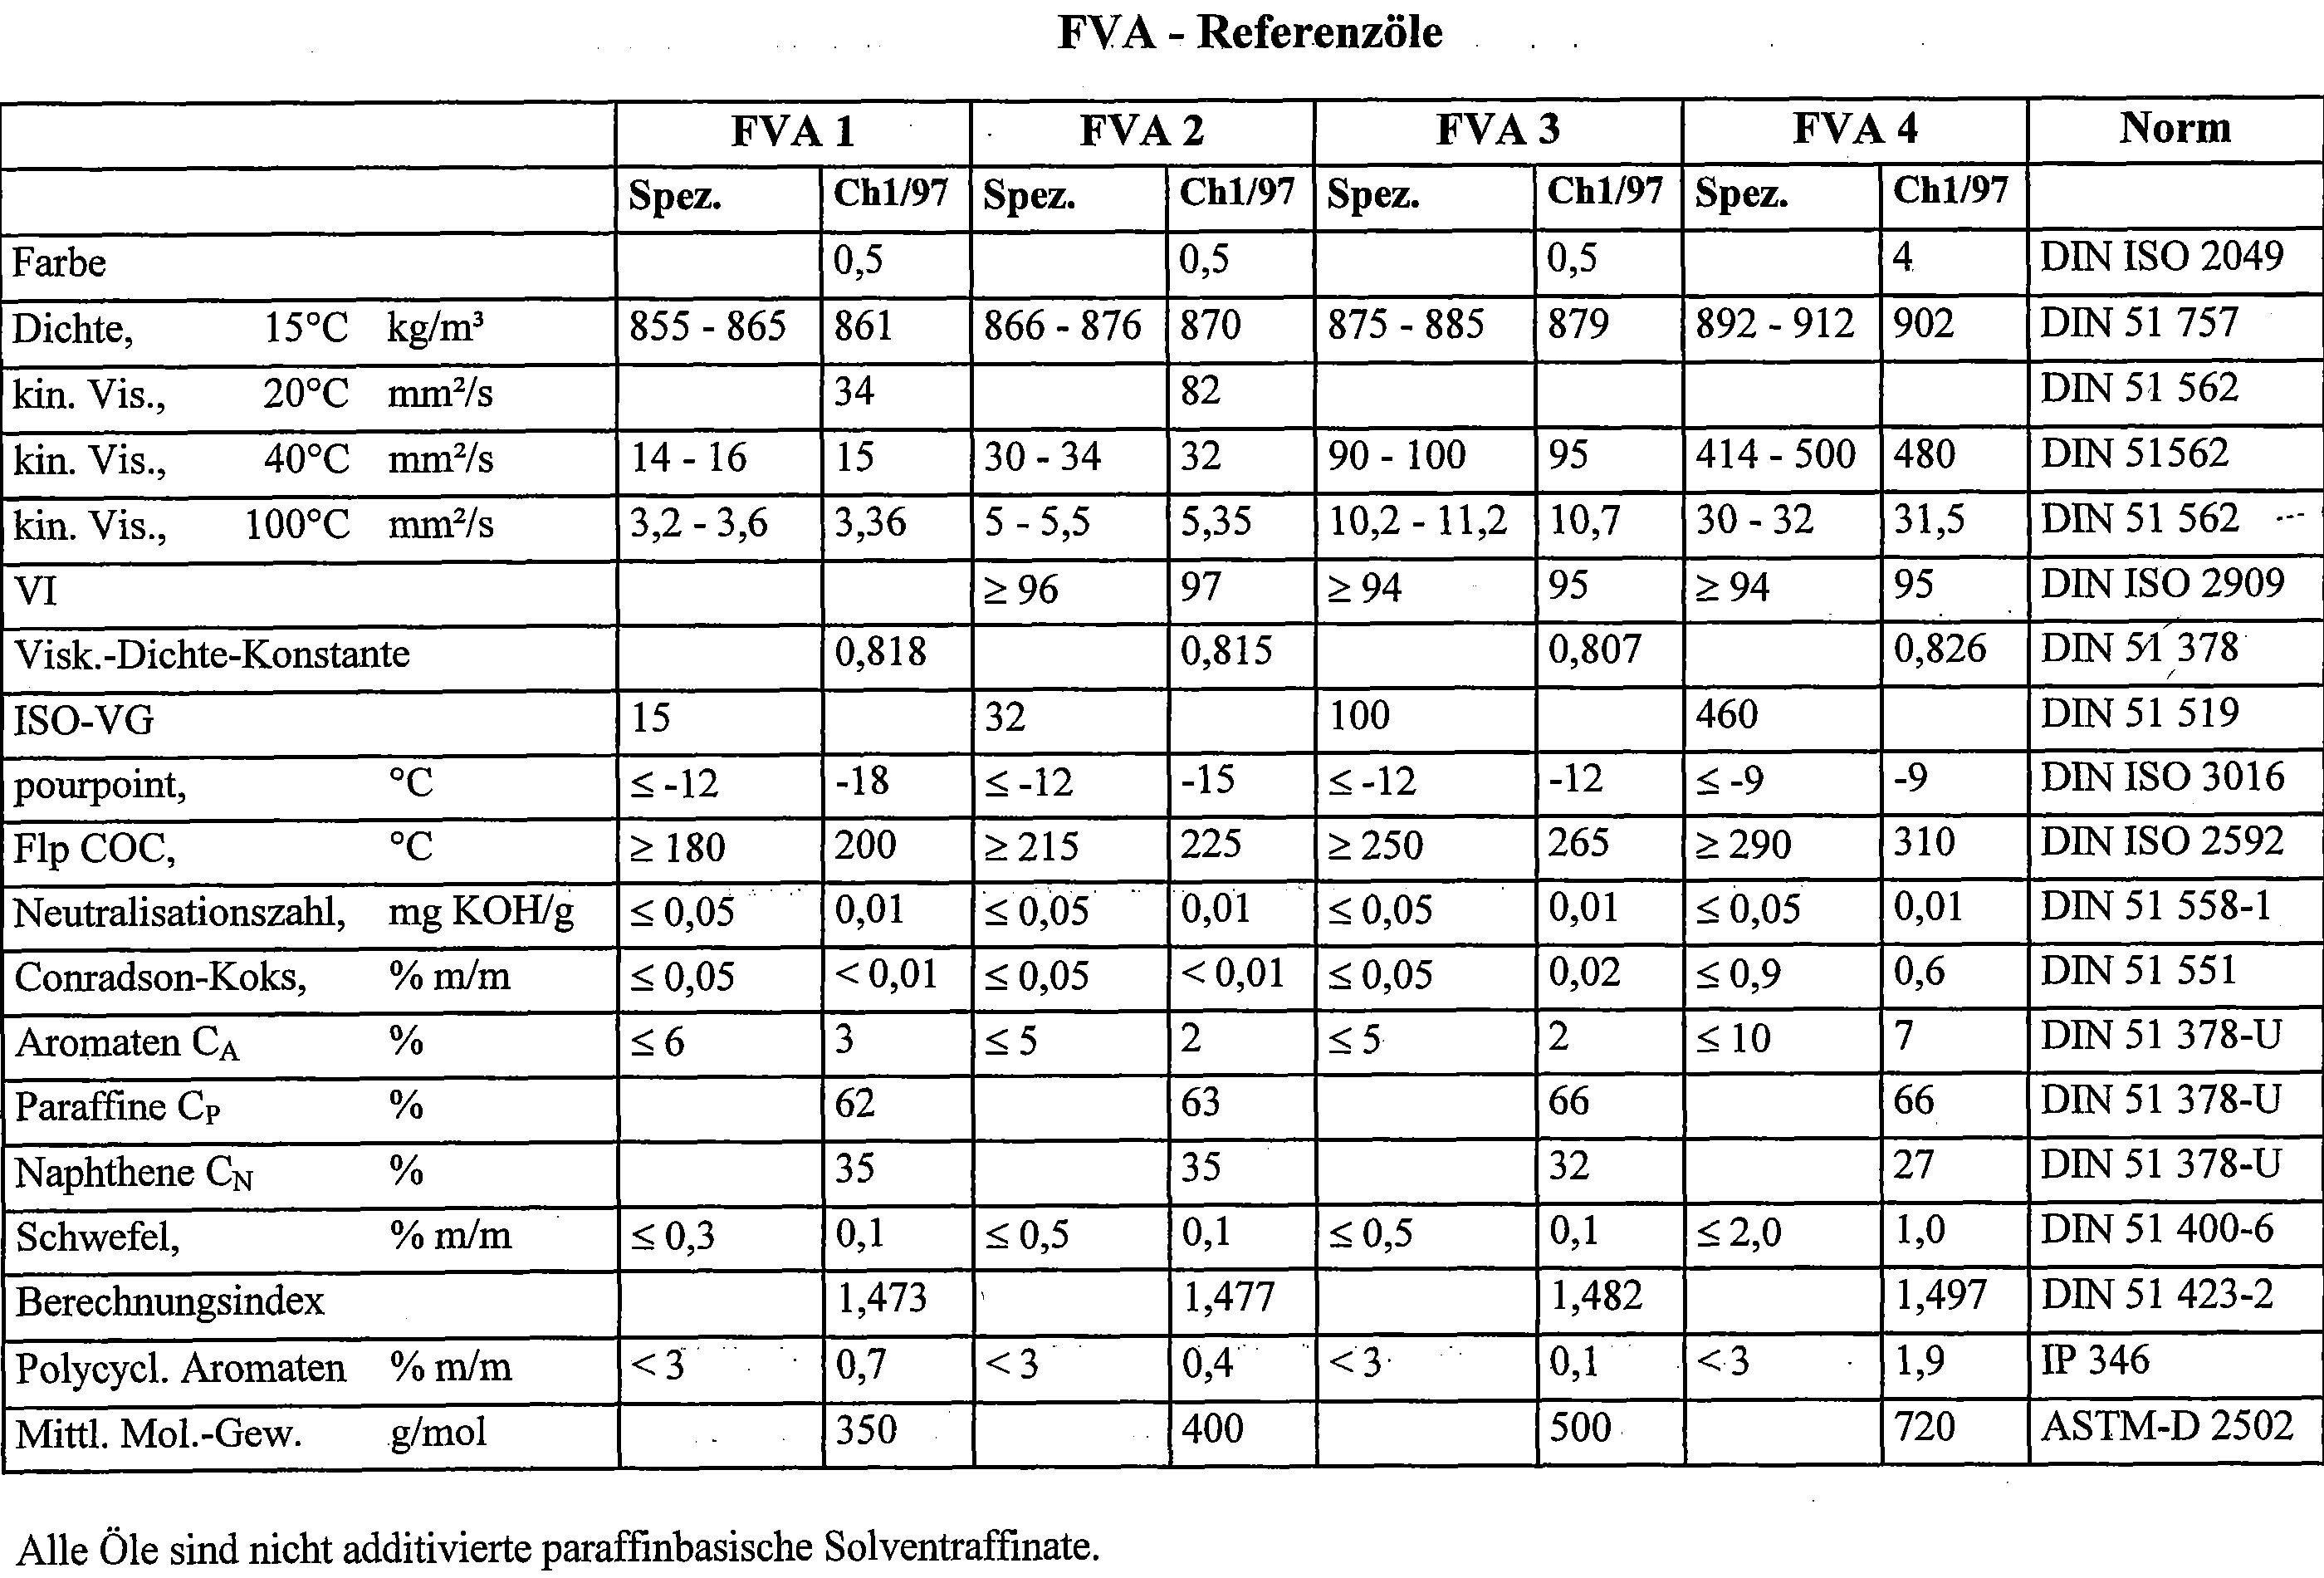
\includegraphics[width=0.9\linewidth]{./images/fva_chemische_daten.png}
            \caption{Chemische Eigenschaften von Referenzölen \cite{schilling_1985}}
            \label{fig:fva_chemische_eigenschaften_referenzoelen}
        \end{figure}

        % ----------------------------------------
        % Fig: FVA Dichte-Temperatur
        % ----------------------------------------
        \begin{figure}
            \centering
            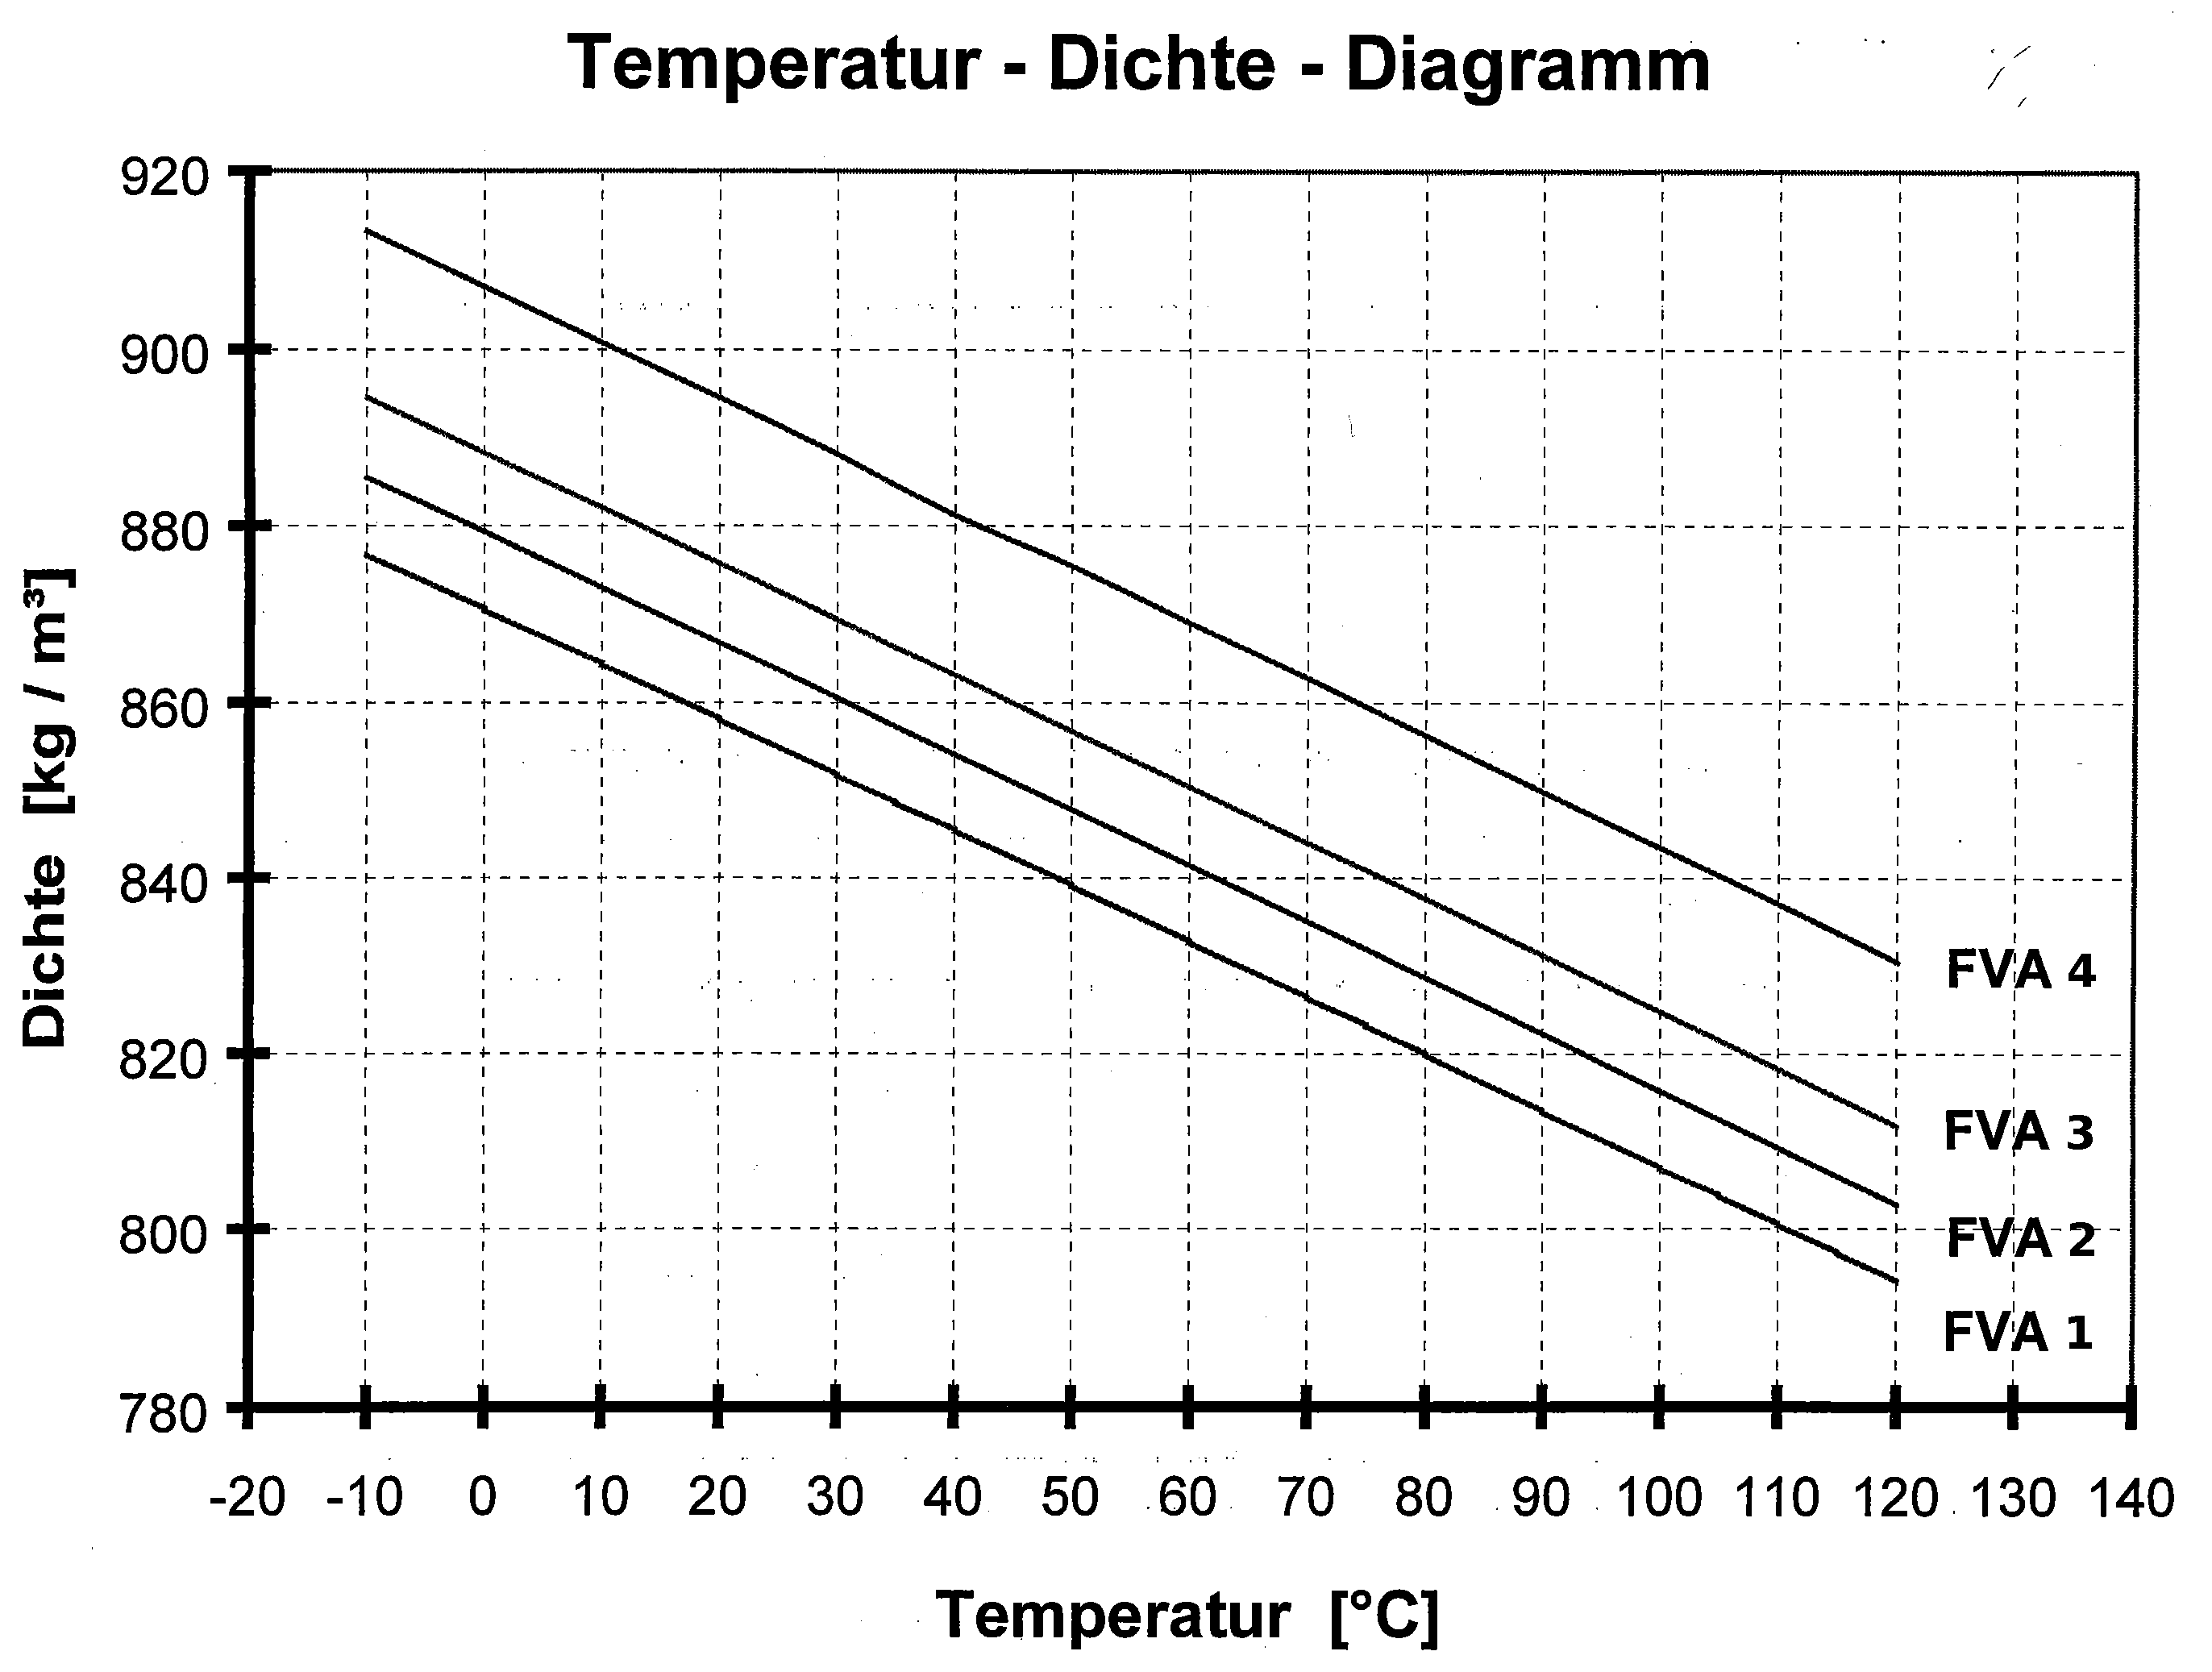
\includegraphics[width=0.9\linewidth]{./images/fva_dichte_temperatur.png}
            \caption{Dichte-Temperatur von Referenzölen \cite{schilling_1985}}
            \label{fig:fva_dichte_temperatur}
        \end{figure}

        % ----------------------------------------
        % Fig: FVA kinematische Viskosität-Temperatur
        % ----------------------------------------
        \begin{figure}
            \centering
            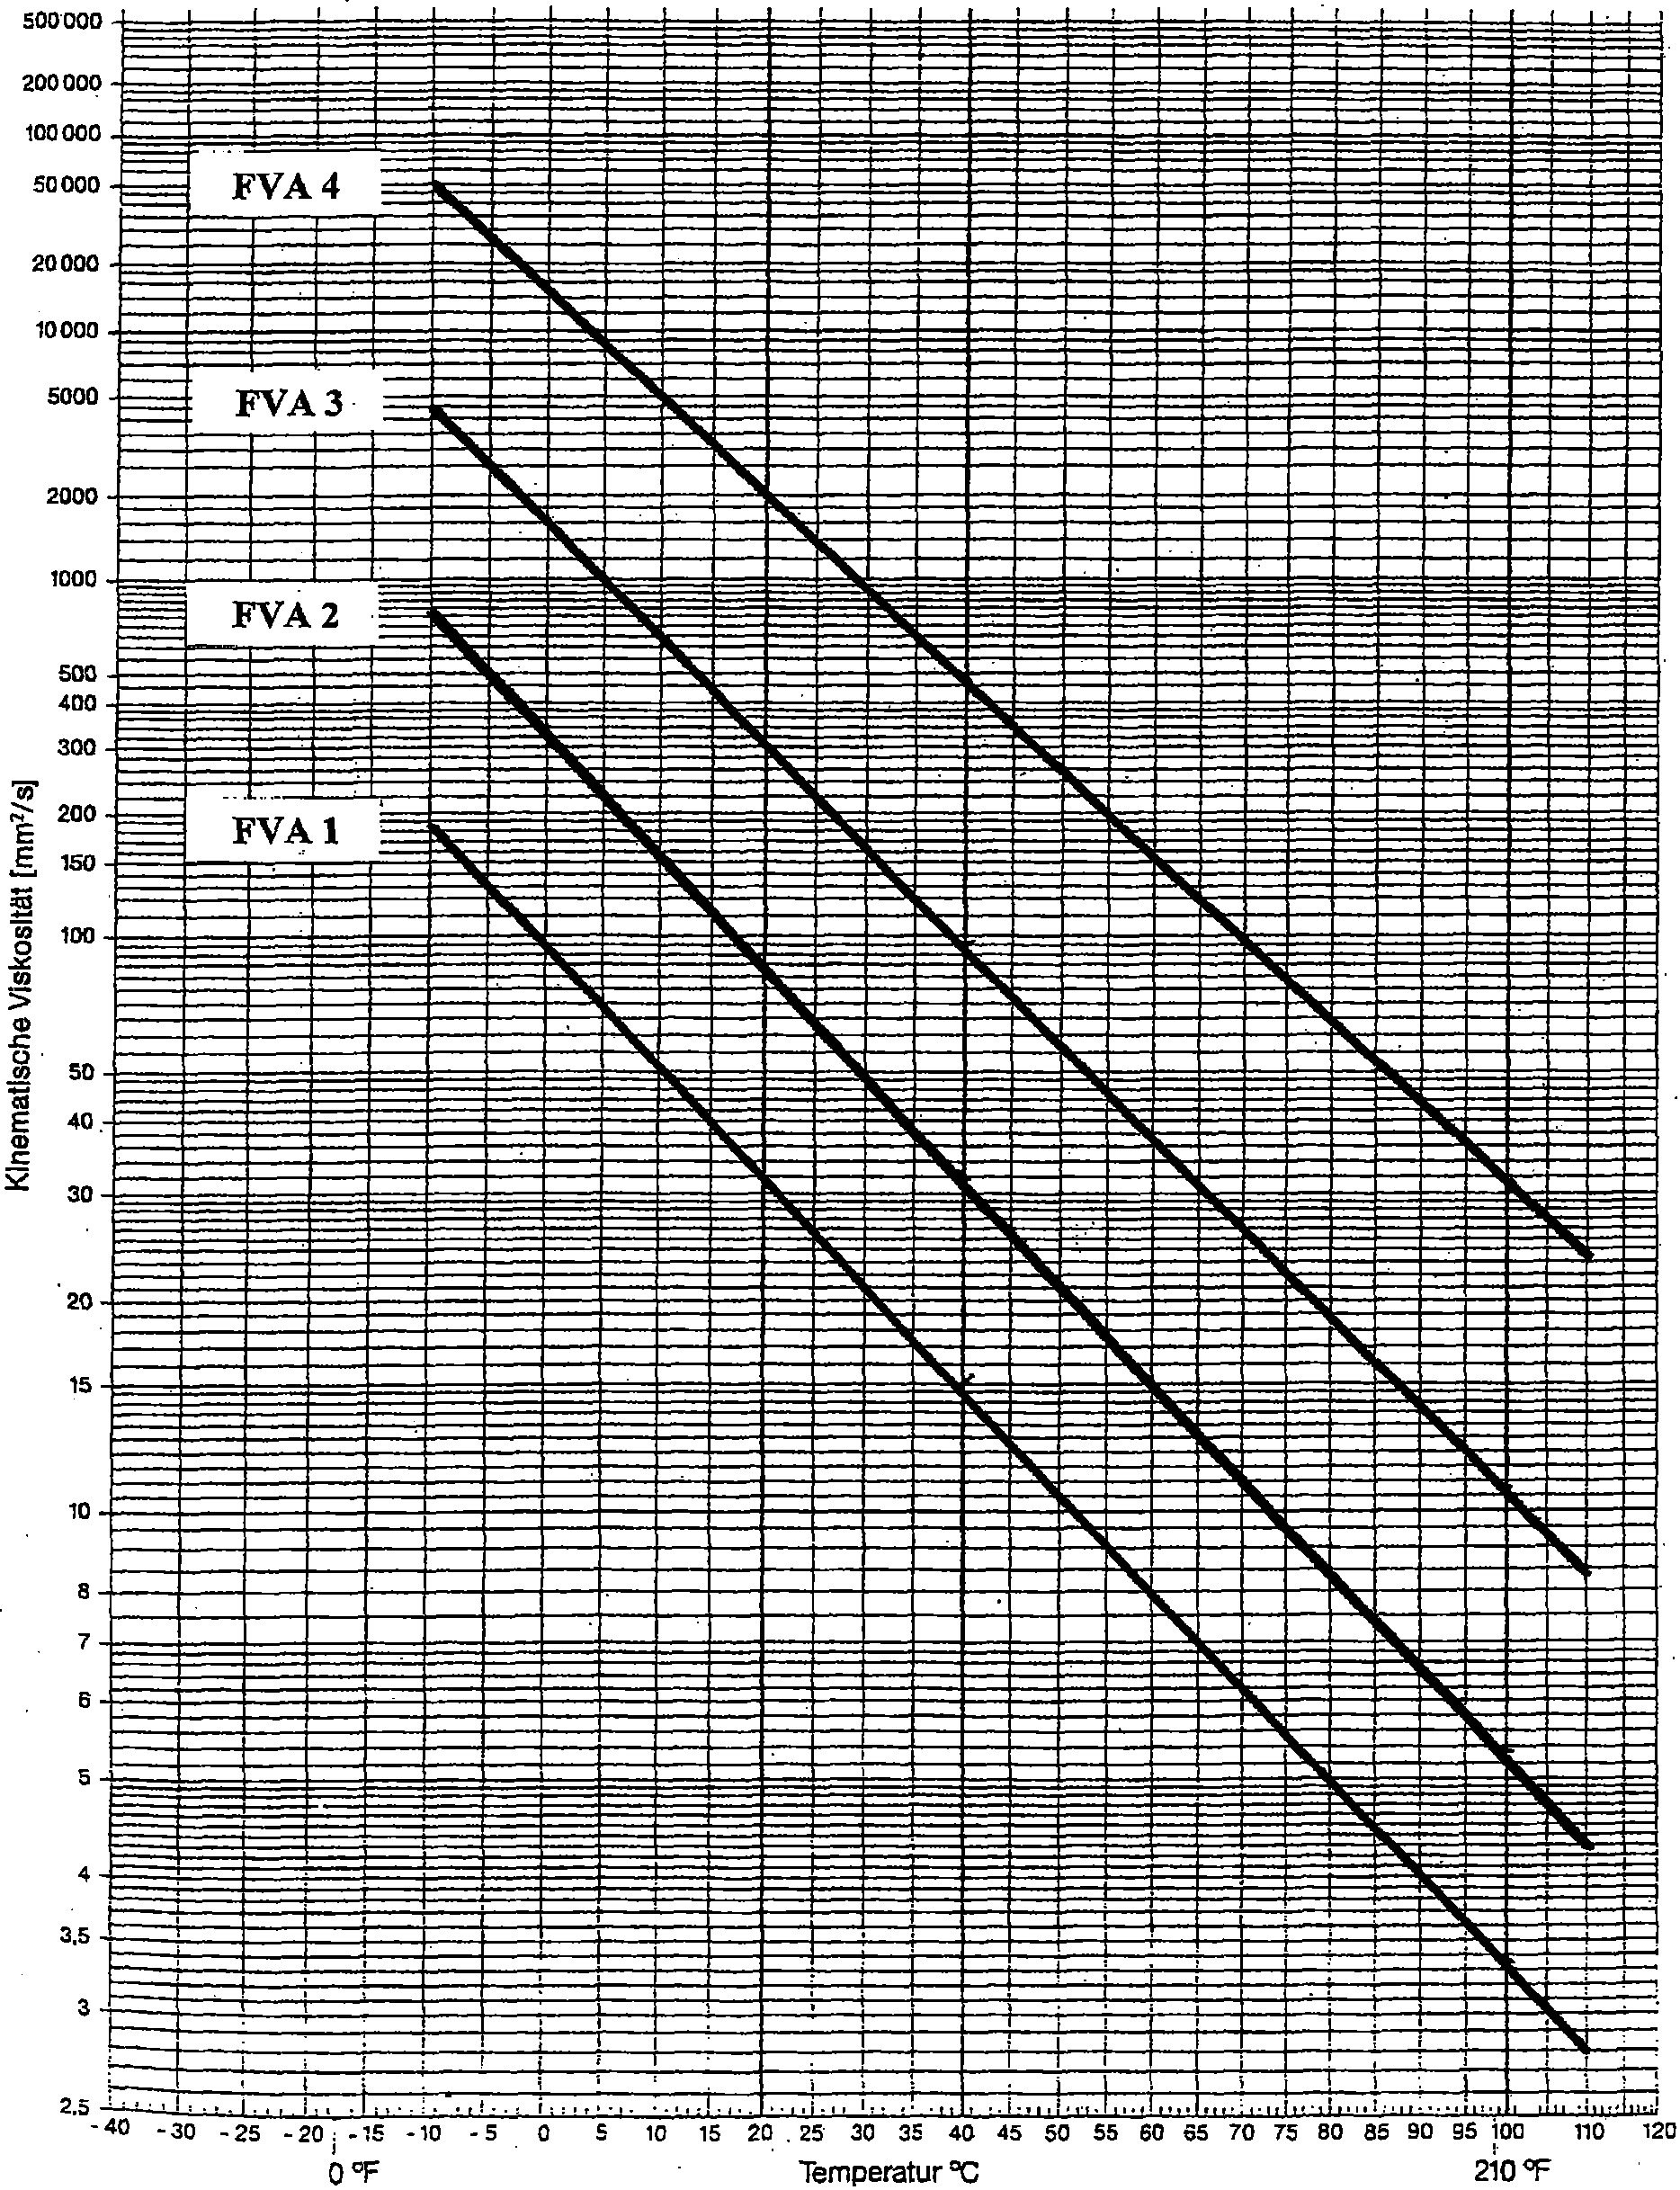
\includegraphics[width=\linewidth]{./images/fva_kin_viskositaet_temperatur.png}
            \caption{Kinematische Viskosität-Temperatur von Referenzölen \cite{schilling_1985}}
            \label{fig:fva_kin_viskositaet_temperatur}
        \end{figure}

        % ----------------------------------------
        % Table: Oil daten
        % ----------------------------------------
        \begin{table}
            \caption{Dynamische Viskosität und Druck-Viskositätskoeffizient der Ölen \cite{esdu_1985}}
            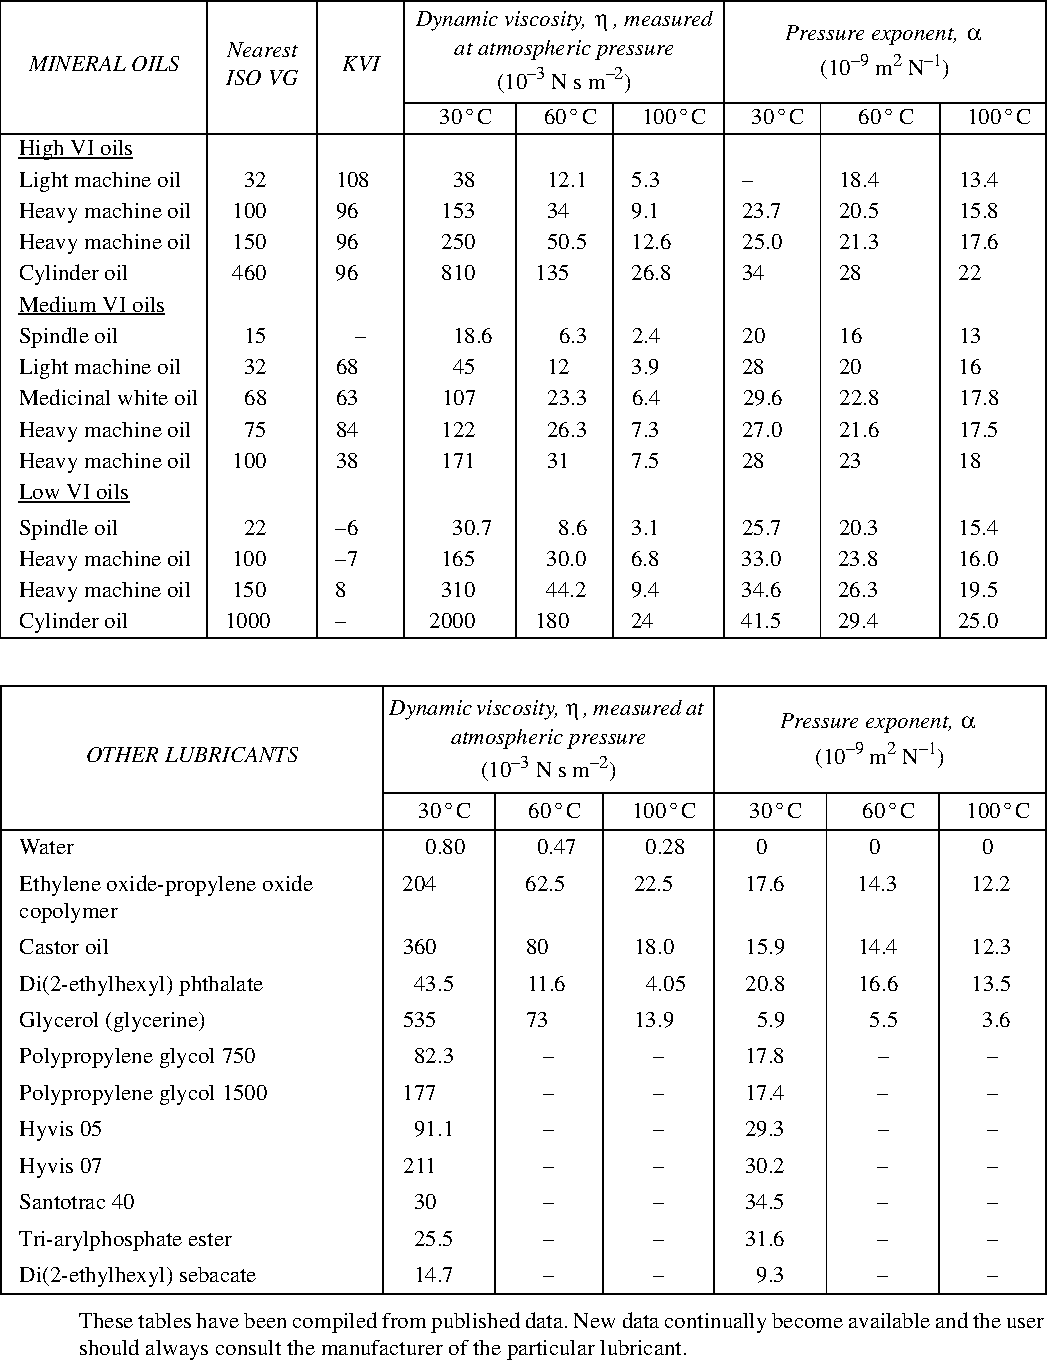
\includegraphics{./tables/esdu_oils_table.pdf}
            \label{tab:esdu_oil_daten}
        \end{table}

    \chapter{PCS EHD-Prüfstand}
    % ----------------------------------------
    % Chap: PCS EHD-Prüfstand
    % ----------------------------------------

    \section{Vorgehensweise für Schmierfilmdicken-Messungen \cite{surborg_2007}}
    % ----------------------------------------
    % Sec: Schmierfilmdickemessung procedure
    % ----------------------------------------
        \begin{enumerate}
            \item PC, Monitor und Bildschirm einschalten
            \item Ultra.exe starten
            \item Elektronikeinheit und Lichtquelle einschalten
            \item Positionen der Temperatursensoren überprüfen
            \item Messtemperatur aktivieren und einstellen: \\
                \textit{Control -> Temperature (Regelung auf Pot)}
            \item gereinigte Kugel und Scheibe einsetzen und mit Rändelschraube sichern
            \item Spritzschutzdeckel auf dem Topf positionieren
            \item Linse des Mikroskops auf Verschmutzung überprüfen
            \item Mikroskop zusammen mit der Lichtquelle montieren
            \item Last aufbringen (\SI{20}{\newton})
            \item grünen Kontaktpunkt im Lichtkreis scharf gestellt und zentriert auf den Spalt ausrichten
            \item \textit{Live} aktivieren
            \item Bild auf dem Bildschirm scharf stellen und dann ausrichten (Z-Achse)
            \item wenn kein Schaden auf der Spur erkennbar ist den Messpunkt festlegen: \\
                \textit{Set -> Trigger Point -> Set Trigger Here}
            \item Messband festlegen: \textit{Set -> Averaging Band}
            \item Testparameter eingeben: \textit{Set -> Test Parameter}
            \item Maximum der 3. Ordnung an den linken Bildschirmrand bringen (Mikrometer ca. \num{0.15})
            \item Mikrometereinstellung und Ordnung in die Software eingeben
            \item \textit{Smooth, Peak Fit, Multiple} und \textit{Auto Add} aktivieren und \textit{Multiple} auf \num{3} Widerholung setzen
            \item Geschwindigkeitsschritte auf \SI{20}{\percent} setzen: \textit{Control -> Speed}
            \item \textit{Immed} drücken
            \item Silikatschicht bestimmen: \textit{Set -> Zero Film}, angezeichten Wert notieren
            \item Last entfernen
            \item die Scheibe ein Stück weiterdrehen: \textit{Set -> Trigger Point -> Jog} (ca. 5x)
            \item verminderte Last aufbringen (je nach Öl, ca. \SI{10}{\newton})
            \item auf \SI[per-mode=symbol]{1.1}{\meter\per\second} beschleunigen und Öl \SI{15}{\minute} durchmischen lassen
            \item Geschwindigkeit verringern und auf \SI[per-mode=symbol]{0.02}{\meter\per\second} einstellen
            \item Last auf \SI{20}{\newton} erhöhen
            \item mit \textit{Trigger} erste Messung beginnen
            \item nach Ermittlung des ersten Wertes wird die Protokoll-Datei angelegt (Name und Speicherort wählen)
            \item mit \textit{Trigger} von \SIrange[per-mode=symbol]{0.02}{4.77}{\meter\per\second} zügig weitere Messwerte ermitteln
            \item erreicht die Ordnung die rechte Bildschirmseite, dann mit Hilfe des Mikrometers zurückschieben oder die nächste Ordnung wählen
            \item übliche Bereich sind: \\
                \begin{tabular}{ll}
                    \SIrange{0}{100}{\nano\meter}       & 3. Ordnung, Mikrometer \num{0.15} \\
                        \SIrange{100}{150}{\nano\meter} & 3. Ordnung, Mikrometer \num{0.16} \\
                        ab \SI{150}{\nano\meter}        & 4. Ordnung, Mikrometer \num{0.14} \\
                                                        & 4. Ordnung, Mikrometer \num{0.16} \\
                                                        & 5. Ordnung, Mikrometer \num{0.15} \\
                \end{tabular}
            \item nach der letzen Messung Geschwindigkeit auf \SI[per-mode=symbol]{0}{\meter\per\second} bringen und Last entfernen
            \item Scheibe zur Überprüfung des Messpunkts ausrichten: \\
                \textit{Set Trigger Point -> Go To Trigger Point}
            \item Last aufbringen (\SI{20}{\newton})
            \item mit \textit{Immed} den Nullfilm bestimmen und den Wert notieren
        \end{enumerate}

    \section{Procedure for resetting the ball track micrometer}
    % ----------------------------------------
    % Sec: Set ball track
    % ----------------------------------------
    The first requirement is to set the 'preset' position on the micrometer to \SI{39.000}{\milli\meter} (the ball track mid position). Do this as follows:

    Ensure the micrometer is operating with the \si{\mm} scale, press the \si[per-mode=symbol]{\inch\per\mm} button if necessary.

    Press and hold down the preset button, the display will change to show \num{000.000}.
    Continue to hold down the button until the second digit begins to flash and then release the button.
    Press and release the button repeatedly.
    The second digit should count up one each time the button is pressed.
    When the number \num{3} is reached, press and hold down the button until the third digit starts flashing.
    Now repeatedly press and release the button until the number 9 is reached.
    Press and hold down the preset button, so that the fourth, fifth and sixth digit flash in turn and then finally the letter $p$ at the top of the display begins to flash.
    Now release the button, press and release briefly.
    The micrometer should now read \SI{39.000}{\mm}.

    The micrometer should now be adjusted to the ball track mid position.
    To do this slacken the loading system lock and gently screw in the ball track micrometer until the ball carriage (bellows assembly) reaches its inner most position.
    Note the reading on the micrometer.
    Now fully unscrew the micrometer, pull out the load system locking bar to ensure the ball carriage is at its most outer position.
    Tighten the loading system lock and gently screw in the ball track micrometer until it makes contact with the ball carriage slide.
    Note the reading on the micrometer, it should be approximately \SI{10}{\mm} greater than the previous reading.
    Now add the two readings together and divide by two, this value $X$ will correspond to the ball track mid position.
    Adjust the micrometer until it reads $X$.
    Press and hold down the preset button until \num{039.000} appears with the $p$ flashing.
    Release the button, press again and release.

    The micrometer should now be reading \SI{39.000}{\mm} in the ball track mid position.
    This completes the setting of the micrometer.
    % ----------------------------------------
    % Fig: PCS Micrometer
    % ----------------------------------------
    \begin{figure}[htb]
        \centering
        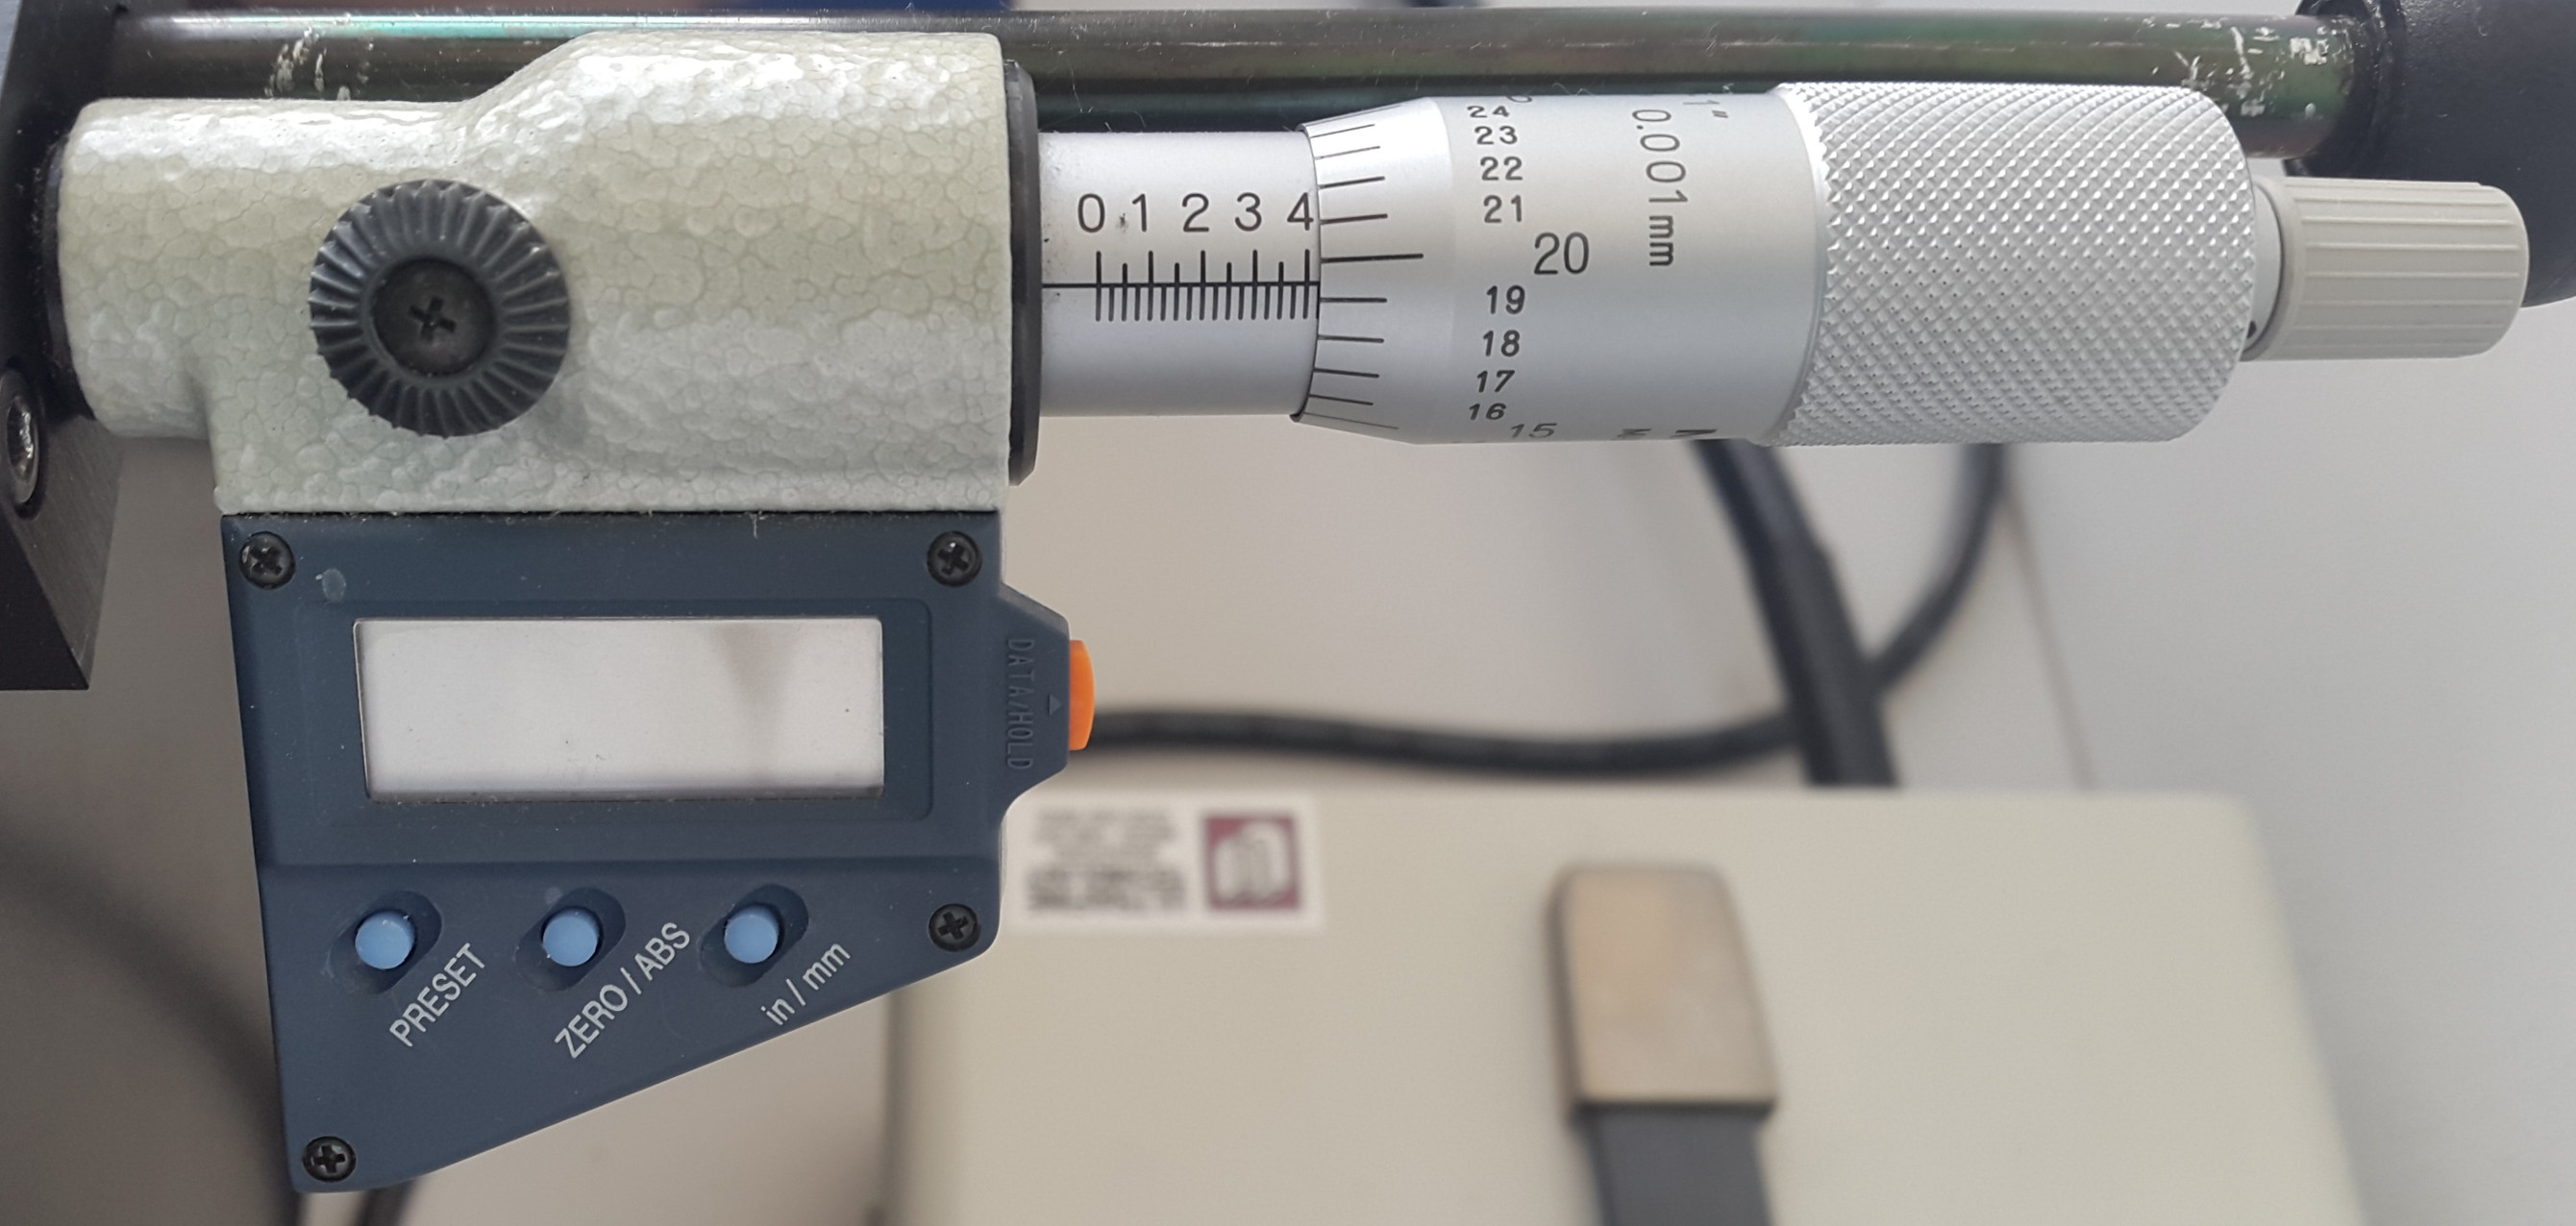
\includegraphics[width=0.8\linewidth]{./images/micrometer.jpg}
        \caption{Micrometer to set ball assembly's position}
        \label{fig:micrometer_ball_assembly_position}
    \end{figure}


    \section{Rauheitsmessung der halben beschichteten Glasscheibe}
    % ----------------------------------------
    % Sec: Rauheitsmessung der halben beschichteten Glasscheibe
    % ----------------------------------------
    \begin{minipage}[b]{0.5\linewidth}
        \centering
        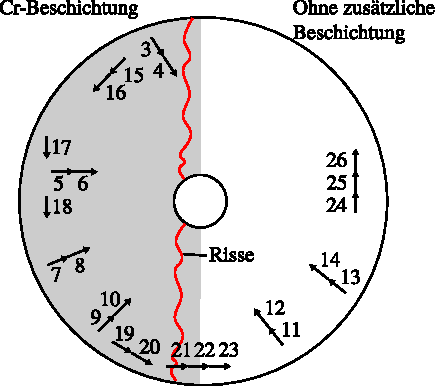
\includegraphics[width=\textwidth]{./images/rauheitsmessung.pdf}
        \captionof{figure}{Messstelle zur Rauheitsbestimmung}
        \label{fig:messstelle_zur_rauheitsbestimmung}
    \end{minipage}
    %
    \begin{minipage}[b]{0.5\linewidth}
        \centering
        \begin{tabular}{rrr|rrr}
    Nr & Ra[\si{\um}] & Rz[\si{\um}] & Nr & Ra[\si{\um}] & Rz[\si{\um}] \\ \hline
    3  & 0.08         & 0.64         & 15 & 0.02         & 0.13         \\
    4  & 0.12         & 0.57         & 16 & 0.04         & 0.38         \\
    5  & 0.02         & 0.16         & 17 & 0.02         & 0.16         \\
    6  & 0.04         & 0.26         & 18 & 0.11         & 0.65         \\
    7  & 0.04         & 0.27         & 19 & 0.02         & 0.12         \\
    8  & 0.03         & 0.21         & 20 & 0.03         & 0.16         \\
    9  & 0.05         & 0.27         & 21 & 0.05         & 0.34         \\
    10 & 0.02         & 0.17         & 22 & 0.02         & 0.12         \\
    11 & 0.07         & 0.38         & 23 & 0.02         & 0.13         \\
    12 & 0.02         & 0.12         & 24 & 0.01         & 0.11         \\
    13 & 0.02         & 0.12         & 25 & 0.02         & 0.14         \\
    14 & 0.01         & 0.12         & 26 & 0.01         & 0.1          \\
\end{tabular}


        \captionof{table}{Rauheit der Scheibe}
    \end{minipage}

    % ----------------------------------------
    % Fig: Rauheitsmessung über die Risse auf der beschichteten Seite
    % ----------------------------------------
    \begin{figure}[htb]
        \centering
        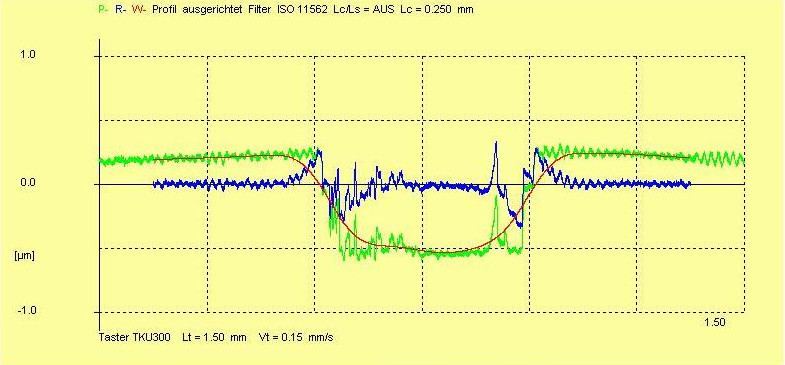
\includegraphics[width=\linewidth]{./images/rauheit_messung_21_plot.jpg}
        \caption{Rauheitsmessung über die Risse zur Bestimmung der Dicke der Cr-Beschichtung}
        \label{fig:rauheitsmessung_ueber_der_risse}
    \end{figure}

    \section{PCS EHD-Prüfstand Spezifikationen}
    % ----------------------------------------
    % Sec: EHL Prüfstand Spezifikationen
    % ----------------------------------------
    \begin{table}[htb]
    \centering
    \caption{EHL-Prüfstand Spezifikationen \cite{ehl}}
    \begin{tabular}{m{5cm}l}
        \multicolumn{2}{l}{\textbf{Kugel}} \\
        Material & \si{Stahl~(100Cr6)} \\
        Durchmesser & $\phi$\SI{19.05}{\milli\meter} \\
        Rauheit Rq & \SI{0.0235}{\micro\meter} \\

        \hline

        \multicolumn{2}{l}{\textbf{Glasscheibe}} \\
        Material & \si{Glas} \\
        Durchmesser & $\phi$\SI{100}{\milli\meter} \\
        Rauheit Rq & \SI{0.033}{\micro\meter} \\
        Spuren & \num{21} \\
        Befahrbarer Radius & \SI{34}{\milli\meter} $\rightarrow$ \SI{44}{\milli\meter} \\
        Beschichtung & \si{Silikat} \\

        \hline

        \multicolumn{2}{l}{\textbf{Motoren}} \\
        Geschwindigkeit & \SI[per-mode=symbol]{1}{\milli\meter\per\second} $\rightarrow$ \SI[per-mode=symbol]{5}{\meter\per\second} \\
        Geschwindigkeit Sprung & \SI{0}{\percent} $\rightarrow$ \SI{100}{\percent} \\
        Schlupf (Kugel-Scheibe) & \SI{0}{\percent} $\rightarrow$ \SI{200}{\percent} \\

        \hline

        \multicolumn{2}{l}{\textbf{Belastung}} \\
        Last & \SI{0}{\newton} $\rightarrow$ \SI{50}{\newton} \\
        max. Pressung & \SI{1.1}{\giga\pascal} \si{(Stahl)}; \SI{0.7}{\giga\pascal} \si{(Glas)} \\

        \hline

        \multicolumn{2}{l}{\textbf{Ölreservoir}} \\
        Volumen & \SI{120}{\milli\litre} \\
        Temperierung & \si{T_{Raum}} $\rightarrow$ \SI{150}{\degreeCelsius} \\

        \hline

        \multicolumn{2}{l}{\textbf{Messsystem}} \\
        Schmierfilmdicke & \SI{0}{\nano\meter} $\rightarrow$ \SI{1000}{\nano\meter} \\
        Genauigkeit & $\pm$ \SI{1}{\nano\meter} \\
    \end{tabular}
    \label{tab:ehl_specs}
\end{table}


    \chapter{Zeichnungen}

\end{appendices}
